\documentclass{article}

\usepackage[utf8]{inputenc}
\usepackage[left=1.5in,right=1.5in,bottom=1in]{geometry}
\setlength\parindent{0pt}
\setlength{\parskip}{1em}
\setcounter{secnumdepth}{0}
\usepackage{outlines}
\usepackage{graphicx}
\graphicspath{ {imgs} }
\usepackage{hyperref}

\title{Urban Economic Geography}
\author{Carla Hyenne }

\begin{document}

\maketitle

\tableofcontents

\pagebreak

%%%%% LECTURE 1 %%%%%

\section{The City as a Social Product}
\date{September 30th, 2021}

There is no such thing as a "pure", "neutral" knowledge or definition of cities/urban space. There are empirical observations, like the density, retail, urban projects, transport, road safety regulations, etc. However, what we see isn't enough. We need concepts, theories, models, abstract tools to make sense of the city.

The type of "intellectual" glasses that we wear influence what and how we understand the space and the issues within it. For example in economics, your views change if you are wearing capitalist vs. socialist glasses.

Thus, what epistemological choices is this class based on? It takes distance from the "urban triumphalism" mainstream, and takes a critical stance on urban issues. 

\subsection{Urban Triumphalism}

Triumphalism depicts cities as a site of progress, a way to prosperity, and we are in a "golden age" of the city. The major \textbf{contemporary challenges} are first urban challenges, and the urban space is where \textbf{solutions} are found. Think of the green, smart, productive, participative, etc., city. 

The key question is then \textit{how} to re-organise the city in order to meet these challenges, by using the potentialities and opportunities in the urban environment. 

\subsubsection{What is the problem with urban triumphalism?}

\begin{outline}
  \1 Urban triumphalism is purely a pro-growth perspective, which is contradictory with the sustainability targets (continuous growth is not sustainable). 
  \1 It is only about finding solutions to a series of pre-defined challenges: how to build the city, equip the city, govern the city, brand the city... This turns urban issues into \textbf{techno-management} issues, where the focus in on the best practices that can be copy/pasted, and where the focus is: 
  \2 on city leaders' views, 
  \2 on best practices for copy/pasting solutions, and 
  \2 on mass production of city rankings which highlight competition

  \1 Consultancy firms (McKinsey) are now targeting the 'CEOs' of cities, that is the mayors, to propose techno-managerial solutions to urban problems. 
These firms are usually focused on maintaining the \textbf{competitiveness} of cities, so that the livelihoods of residents are maintained. This statement from McKinsey is contradictory, since most residents are not involved in making the city competitive, and could be better off if cities were less capitalist.

The mass production of city rankings, also done by consultancy firms, are not transparent. They emphasise the importance of competition amongst cities

  \1 There is a strong inclination towards \textbf{reification} (treating something immaterial, as a material thing). 
  	\2 The social objects are conceived as a mere thing, a coherent and active whole. Cities are viewed as actors
	\2 The city is viewed as an actor ("the city does this"), and acts according to a series of shared interests and aspirations. However, what is good for one is not always good for the other (usually, what's good for businesses/elites is not good for the rest) 
\end{outline}

Marcuse, in \textit{The City as a Perverse Metaphor} explains that seeing the city as an actor excludes a set of the population who does not share the same interests and aspirations. Not all the city is international, competitive, and so on, even if some firms, some people might be. 

\subsubsection{Breaking with Triumphalism}

\begin{outline}
	\1 The city is not an actor, but a \textbf{dynamic space} where actors with different resources, interests, aspirations, interact in diverse ways, from open conflict violence to resistance, mobilisation, collaboration, solidarity
	\1 Urban issues are not all \textbf{techno-managerial} ones, but also \textbf{political}
		\2 Urban space are composed of an established web of social relations, sedimented through history in a specific geographical context
		\2 Urban change is therefore fundamentally conflictual, regarding material forms, norms, regulations, symbolic landscapes... (these are political conflicts, where disagreement and lack of consensus is the default)
		\2 Thus, \textbf{urban landscapes are dynamic and contested landscapes of social power}\footnote{Example: the Berlin referendum on collectivisation, to decide who decides on the rent of the city. This shows the politicisation of an urban space, where a group of individuals use their social power to contest regulations.}
\end{outline}

\subsection{Critical urban studies}

\subsubsection{Definition}

Critical urban studies are
\begin{outline}
	\1 Contra \textbf{naturalising} views: there is nothing natural about cities, how they are shaped, built, transformed, governed, represented. They are not a "living organism"
	\1 Contra \textbf{techno-managerial} takes on urban issues: focus instead on tensions and contradictions, and not solutions to standardised challenges
\end{outline}

Cities are not permanent, but \textbf{dynamic force fields, shaped by social forces, acting through complex set of actors embedded in historically and geographically situated configurations of power relationships.}

Critical urbanism started in the 1960's in the US, because the existing theoretical frameworks could not explain what was happening on the streets:

\begin{outline} 
	\1 Detroit 1967: 1967 Detroit riots, confrontation of black residents and Detroit police)\footnote{"Social Justice and the City", David Harvey} 
	\1 Bruxelles 1969: La Marolle protest, by residents against plans to expand the justice palace into the Marolle quartier 
\end{outline}

\subsection{The production of urban space}

Urban space can, and has been, produced differently. It often gives insights in to the type of society who lived there

\begin{outline}
	\1 Hierarchical society: Nuremberg 15th century. A castle with a moat suggest feudal society, the city walls suggest a violent society
	\1 Agricultural, centralised, rural society: fictional rendition of Babylon, the power is concentrated in a city within the city
	\1 Colonial society: Santiago de Chile, 16th century. The grid guidelines typical of Spanish colonial development
	\1 Industrial society: Roubaix, 20th century. Villes-cheminées (stacks), where work, home, leisure spaces were in the same place\footnote{Friedrich Engels, "The Condition of the Working Class in England"}
\end{outline}

In each society, spatial configurations are organised a specific, non-arbitrary ways, in the image and in support of a particular \textbf{social order}. A soviet (or post-soviet) city, with large boulevard/impressive and brutalist architecture is organised differently from capitalist American cities.

For any society at different moments in time, ordering its space (material, function, political-administrative, symbolic dimensions) is as crucial as organising its production system, its political/legal framework, its cultural/ideological/estethic norms...

\subsubsection{Production of space today}

What picture should we paint to describe the society of today? Landscapes of skyscrapers, or slums and inequality, private or public space (or privatised public space?), of consumption, blurred boundaries, planetary dimensions, transportation and networks?

There are many landscapes: skyscrapers of Doha, skyscrapers vs. disinvested neighbourhoods of Detroit showing sharp inequalities, the ultra libertarian and capitalist Space X with no state regulation.

\subsubsection{Heuristic of the production of urban space}

\begin{outline}
	\1 Move \textbf{from an essentialist, to a relational thinking} about cities. Cities do not have a set of attributes that are necessary for them to "a  city". The object is not 'the city', but the dynamic relationships of societies to urban space. 
	\\\textit{Relational thinking: cities as social products}
	\1 Move \textbf{from a historical to a diachronic thinking} about cities. The production of space is always a "work in progress", through which inherited socio-spatial configurations are reshaped according to new logics. That is, the urban spaces in a \textit{permanent flow of creative destruction}
	\\\textit{Diachronic thinking: cities as "work in progress"}
	\2 Examples of impermanent, in progress urban landscapes: 
		\3 Place De Brouckère, Brussels: project to remove traffic from the boulevard, and undo the work from the 60s where axes of transit (automobile) were built in to the city, and people were de-prioritised. 
		\3 Senne, 19-20th century: Haussmann copy/paste urbanism approach was adopted in Brussels and the Senne was covered up.
\end{outline}

Some questions are barely addressed, if not avoided, by mainstream managerial-like takes on cities:

\begin{outline}
	\1 For/against whom is the city built, planned, renewed?
	\1 According to what kidn of ideology or development model?
	\1 Which social forces are responsible for the permanence or deepening of profound inequalities between/within cities?
	\1 Who has a voice when making decisions about urban projects/policies?
	\1 Who decides how cities are shaped?
\end{outline}

In the 1960s-70s, Henri Lefebvre, a Marxist philosopher, was a leading figure in critical urban studies ("The right to the city", "The production of space"). Lefebvre asks, \textbf{who produces the city, and how?}. His contributions are

\begin{outline}
	\1 An extension of Marx's thoughts: \textbf{any political economy implies a specific spatial order}. That is, the capitalist mode of production relies on particular spatial configurations, adapted to its structural purposes of capital accumulation implying permanent growth
	\marginpar{We have capitalism by design, and our cities can be reorganised differently}
	\1 \textbf{A materialist take on cities}. What are the urban/spatial conditions for each type of political economic system? How are they settled and reproduced?
	\1 \textbf{Not limited to material dimensions}. That is, not only the built environment, but also the norms, regulations, ideologies, techniques, sumboles, values, myths...
	\1 Attempt to \textbf{politicise urban issues}, because the urban is where social struggles happen. Social struggles must appropriate a space\footnote{2021 Berlin rent collectivisation movement}
\end{outline}

All in all, Lefebvre's is a politically-loaded theorisation. The urban space is the terrain of social struggles, but also has a stake in these struggles.\marginpar{Social struggles are urban struggles}

Brenner and Schmid (2015) call for a new "new epistemology of the urban", where the urban fabric is dynamic, evolving, with three moments of urbanisation interacting to produce socio-spatial organisation and uneven development. These three moments are: concentrated urbanisation, extended urbanisation, differential urbanisation.

All of these urban landscapes and processes interact, to produce the urban fabric of the world.

\begin{outline}
	\1 \textbf{Concentrated Urbanisation}: spatial clustering of population, means of transportation, infrastructure, investment
	\1 \textbf{Extended Urbanisation}: activation and transformation of places, territories, landscapes in relation to agglomeration processes; subsequent uneven thickening and stretching of an urban fabric across the planet
	\1 \textbf{Differential Urbanisation}: relentless creative destruction of 'implosion-explosion' of socio-spatial organisation; production of new urban 'potentials' for the appropriation of the extant urban configurations and for the production of radically new forms of urban space
\end{outline}

\subsection{A map of the course}

City as social product $\rightarrow$ Influence of capitalism $\rightarrow$ Governance $\rightarrow$ Everyday life

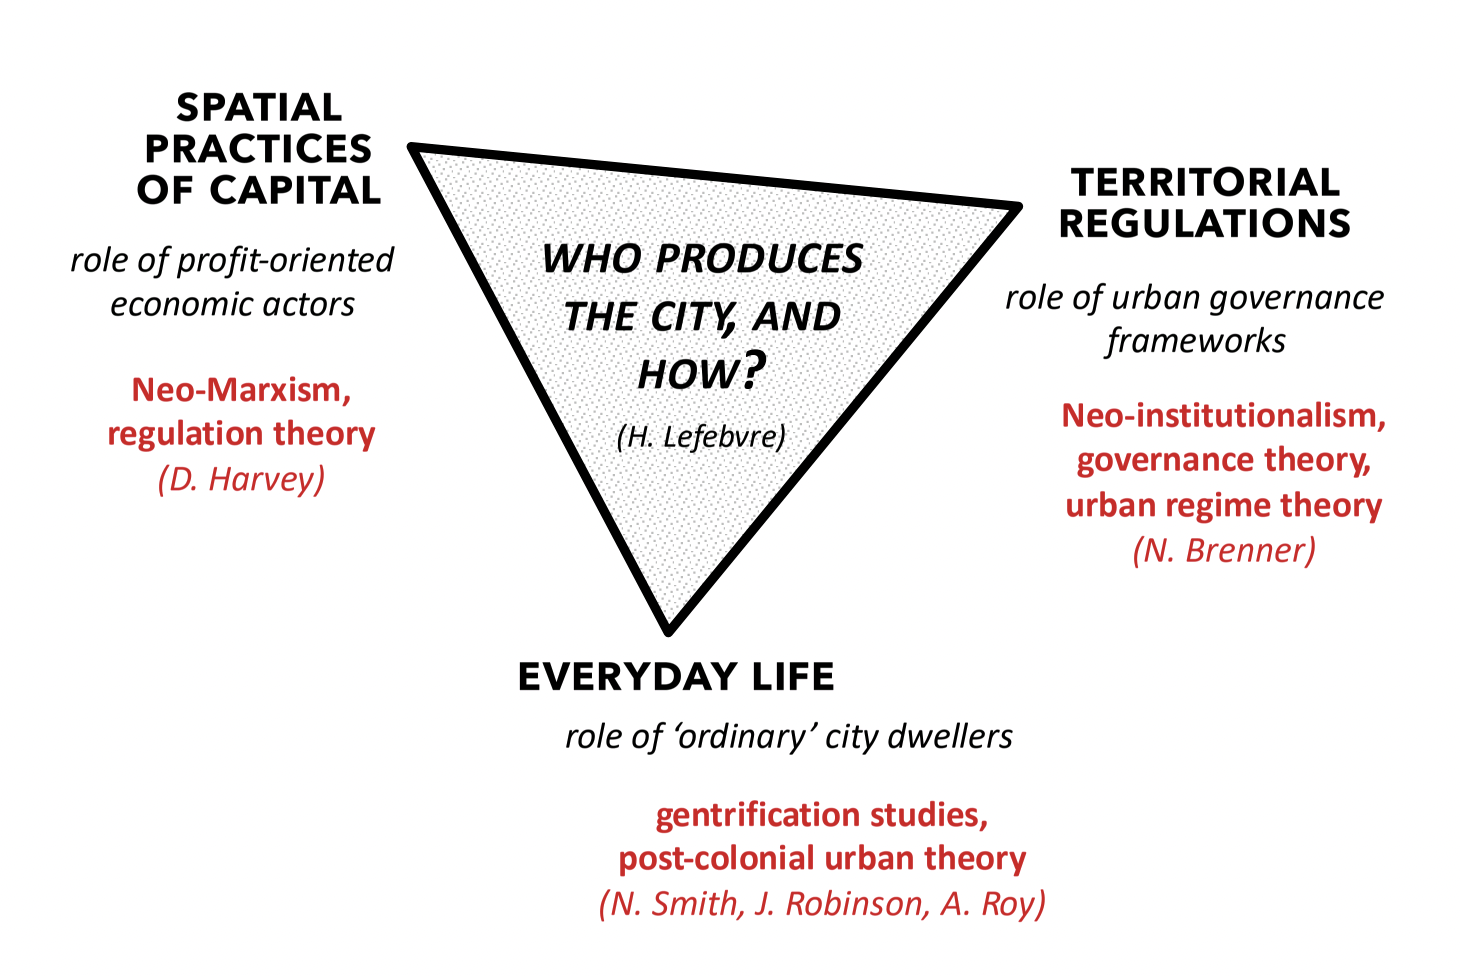
\includegraphics[width=\textwidth]{map_course_organisation1}
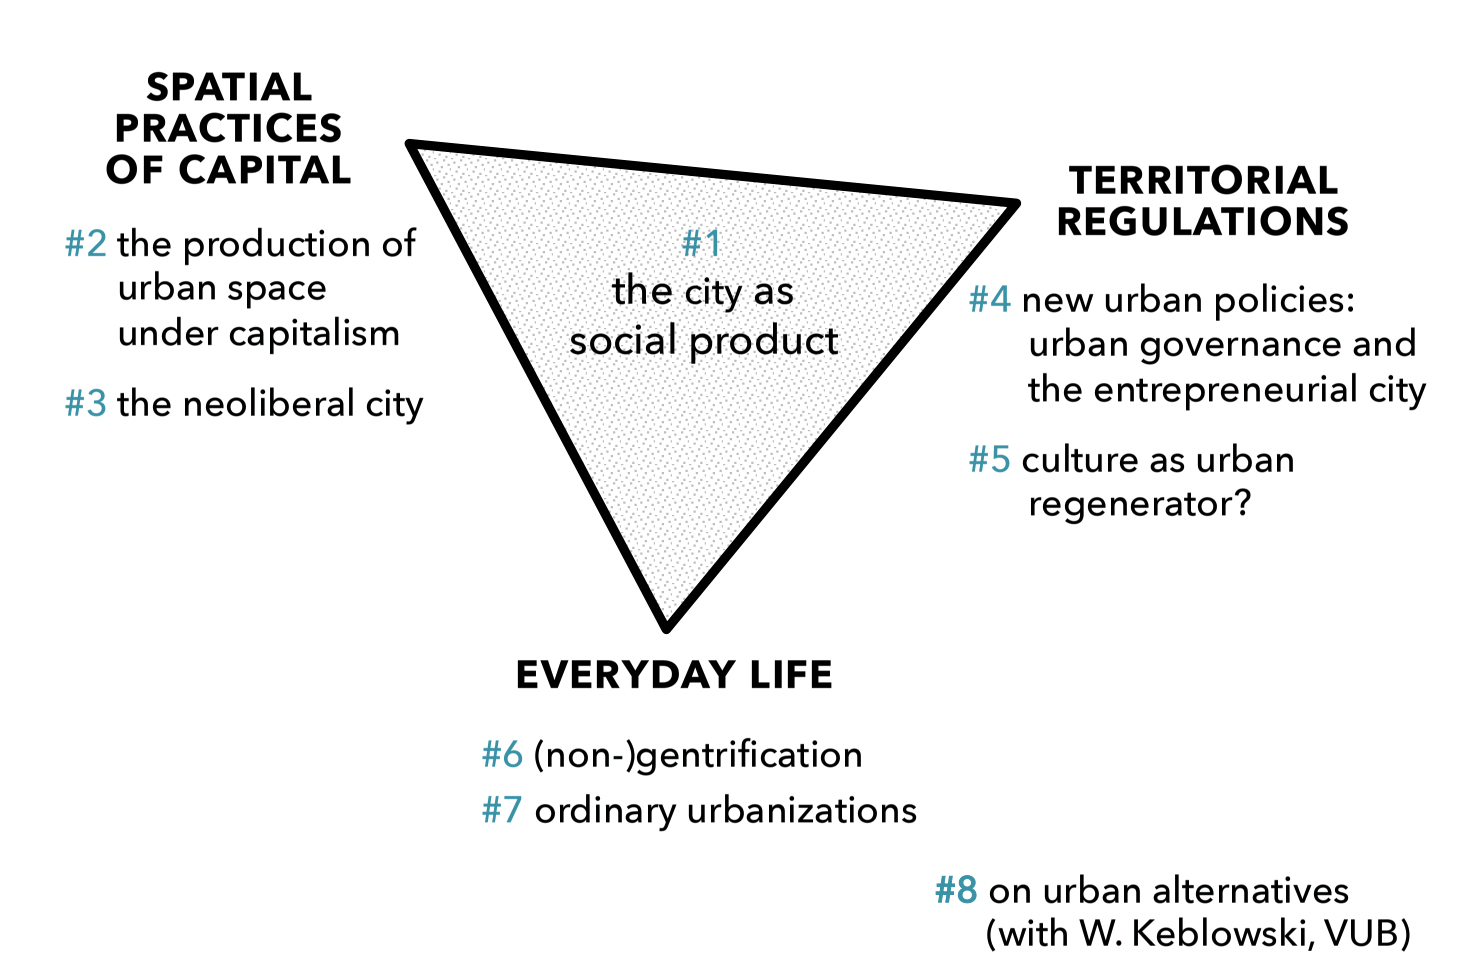
\includegraphics[width=\textwidth]{map_course_organisation2}



%%%%% LECTURE 2 %%%%%

\section{The Production of Urban Space Under Capitalism}
\date{October 7th, 2021}

\textit{tldr; Harvey's theory of the production of urban space under capitalism}

\subsection{Evolution of Urban Space}

What do you think about when you think of urban landscapes? $\rightarrow$ standardisation and copy/past urbanism, shopping streets, high streets; gated communities, suburbanisation, landscapes of dispossession; Dubai, skyscrapers, American malls with extensive parking lots; inequality landscapes; CBD (Central Business District)

We could think of:

\begin{outline}
	\1 Shanghai: from 1990 to 2014, it became a metropolis, China entered the world trade organisation and became a super power
	\1 Panama City: from 1930s to 2010s, became a haven for tax-evasion and offshoring of wealth; came to light with Panama papers
	\1 Cleveland Ohio: in 2008, had many foreclosures due to financial crisis, landscape of abandonment and dispossession 
\end{outline}

\subsubsection{David Harvey}

David Harvey had a theoretical project \textbf{``to integrate an understanding of processes of urbanisation and built environment formation into the general theory of the laws of motion of capital''}, ie. how does urbanisation help us understand capitalism.

He asks the questions:

\begin{outline}
	\1 How and why does capitalism (re)shape (urban) space?
	\1 What's structural about the urbanisation of capitalism, and what's historically/geographically contingent?
	\1 How does the restless character of capitalism (crises, booms, busts...) affect cities?
	\1 How and why does the capitalist production of space bring uneven spatial development?
\end{outline}

\subsection{Capitalism and urbanisation}

\subsubsection{Capitalism}

Capitalism is a system of economic production based on the circulation, or exchange, of privately-owned capital and geared towards capital accumulation. 

Under capitalism, you must re-invest your profit, otherwise other actors will out-compete you (and put you out of business). You also want public or private investors to invest in your business, and such financial investments have grown so much as to become problematic\footnote{The financial investment space is not something I understand well; general understanding is that banks, or finance institutions, lend money/invest, ie. give credit, which means the businesses/people must pay back this money plus interest, and this means they must make a profit. And this has become a problem, because loans cannot be paid back correctly or on time?} 

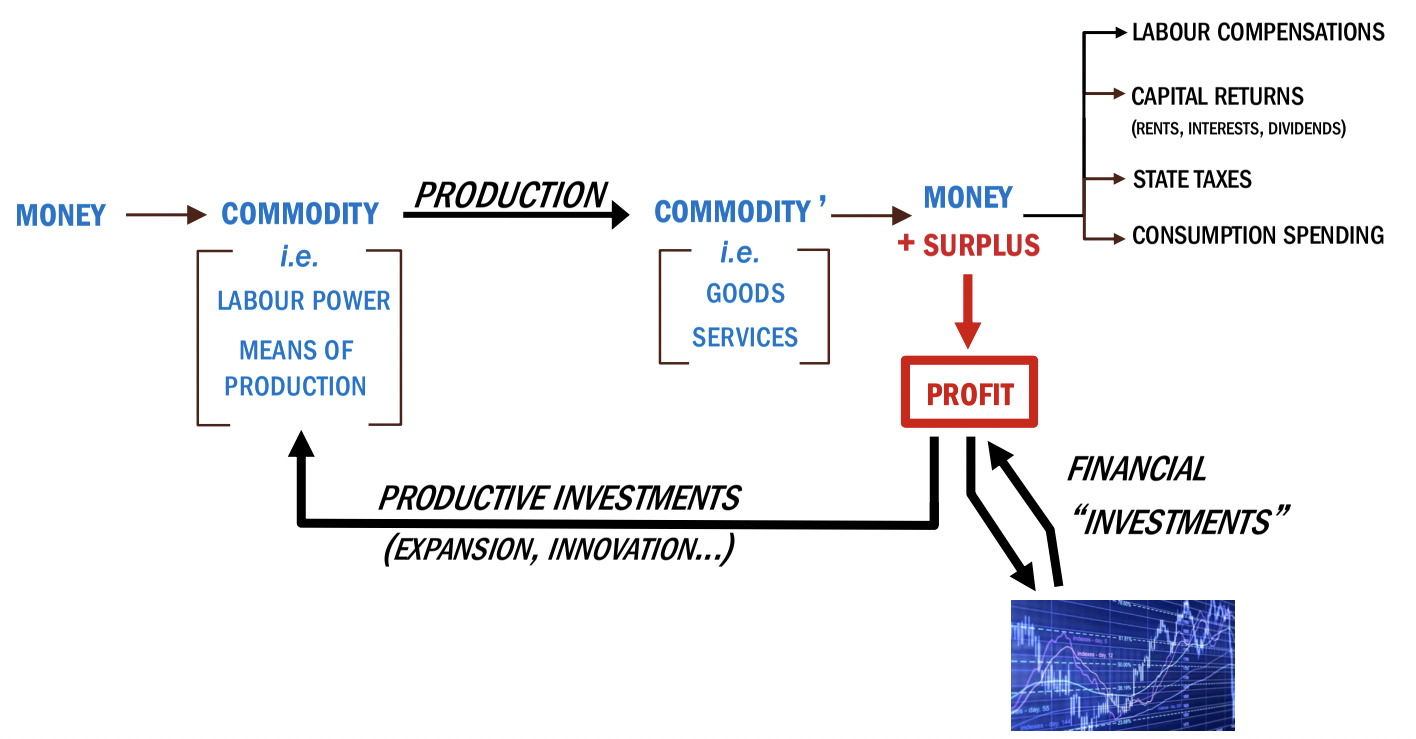
\includegraphics[width=\textwidth]{capitalism}

Thus, capitalism:
\begin{outline}
	\1 An ever-expanding system: capitalism must grow
	\1 Has a geography: it isn't the same everywhere, it's embedded in varying social, cultural, institutional configurations (eg. colonial capitalism, war capitalism, State-controlled capitalism...)
	\1 Has a history: it evolved over time, from a merchant capitalism (16-17th century) $\rightarrow$ liberal industrial capitalism (18-19th century) $\rightarrow$ Fordist/Keynesian industrial capitalism (20th century) $\rightarrow$ neoliberal capitalism (late 20th century)
\end{outline}

%\subsubsection{Capitalism and urbanisation} 

Can we say that cities are created by capitalism? No, cities are not creations of capitalism and existed prior to it. However, the rise and extension of capitalism is deeply linked to the urbanisation process: the emergence of merchant capitalism in Europe's medieval cities, and the massive urban transition since the rise of industrial capitalism, are two eras where capitalism sped up urbanisation.

\subsubsection{A crisis-prone system}

Capitalism is crisis prone, but it has been resilient through history\footnote{China's Evergrande crisis: the collapse of China's second biggest property developer created fear that China's financial system could collapse, however, it did not.}. 

\begin{outline}
	\1 Accumulation is at risk when surplus capital has no outlet in sight for profitable reinvestment, because the circulation of capital cannot continue
	\1 If an outlet is not found, the financial bubble crashes, there are plant closures, social upheavals, geopolitical conflicts...
\end{outline}


Harvey focuses on capitalism's crises. His guiding question is, throughout history, how has capitalism emerged from its periodic crises and found ways to expand further?

\subsection{A theory of urbanisation under capitalism - `fix'}

A `fix' can be one of three things: to put something in place; to repair something; to satisfy an addiction. In capitalism, a fix is a \textbf{temporary `solution' to capitalism's inner crisis tendencies.}

\textbf{Technology fix}: reinvestment of surplus of capital in new or improved production capacities, ie. new sectors and products fuelled by technological and organisational innovations $\rightarrow$ new rounds of growth

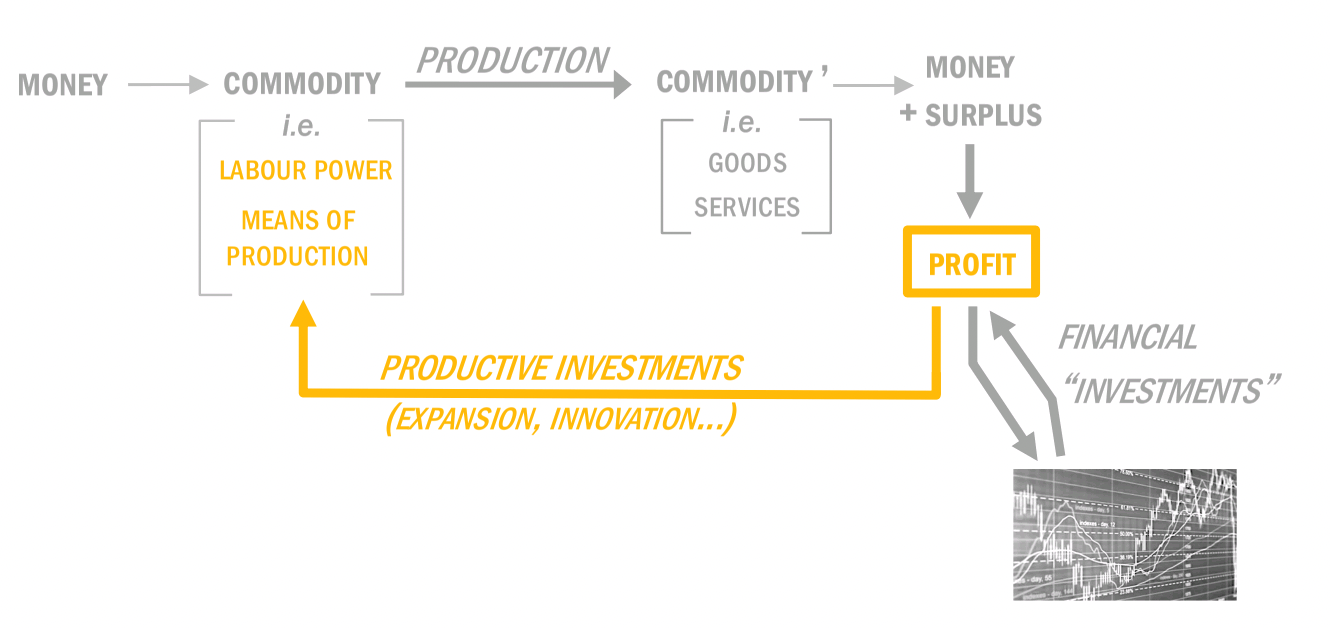
\includegraphics[width=\textwidth]{technological_fix}

\textbf{Financial fix}: reinvestment of surplus capital into financial assets (shares, securities, debt claims...) for the sake of rents and capital gains. This is `financialisation' of capitalism\footnote{For financialisation of capitalism, refer to class no. 3}

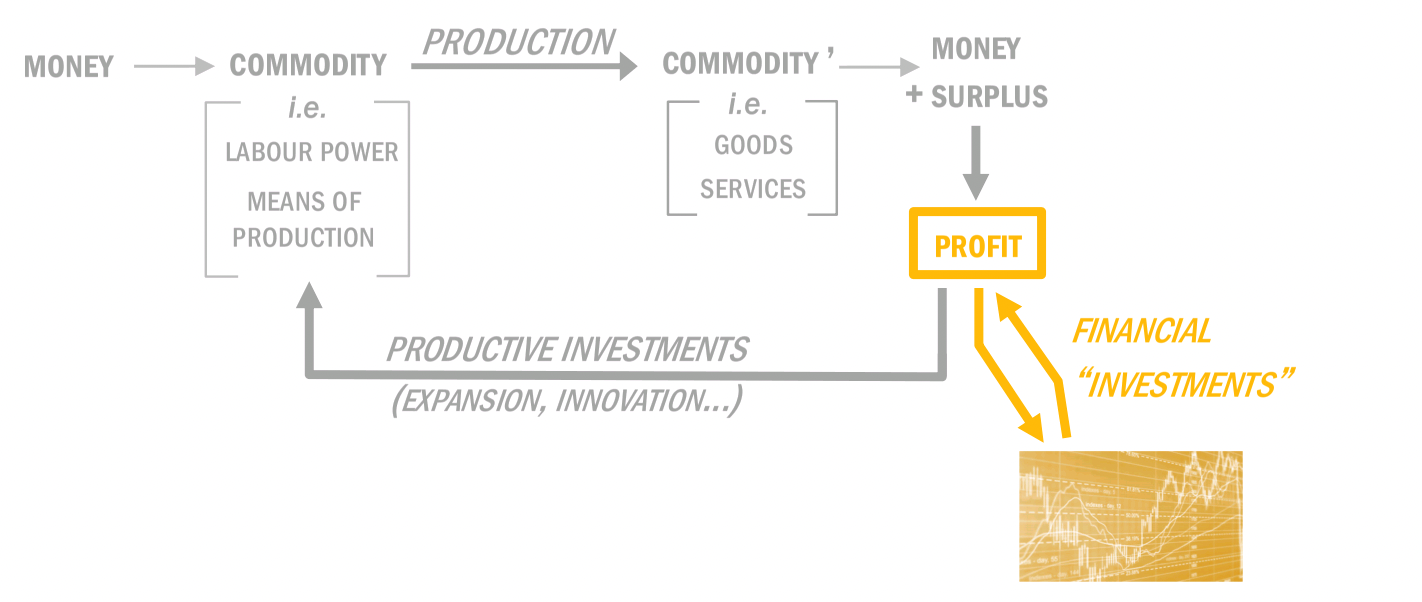
\includegraphics[width=\textwidth]{financial_fix}

\textbf{Spatial fix}: injecting surplus capital into the production of profitable investments. We can observe that the peaks of the construction of tall buildings are not randomly distributed, and are higher at times of crisis (1930s, early 70s, late 80s-90s during the dot com crash and its over optimism, 2008 subprime mortgage crisis).

China and the UAE have the highest number of skyscrapers, and at the same time are places where massive capital surplus exists (or existed at time of building).

\subsubsection{A theory of urbanisation under capitalism}

\begin{enumerate}
	\item Volumes of capital are invested in a selection of localised built environments, in sync with macro-economic temporalities
	\item There is a paradox: investment volumes in the built environment peak in crisis time
\end{enumerate}

Harvey's point is that under capitalism, urbanisation is essential to over capitalism's inner contradictions. \textbf{The production of space is a key outlet for surplus capital and profitable reinvestment} (= spatial fix). ``Capitalism ... is addicted to geographical expansion much as it is addicted to technological change and endless expansion through economic growth''.

The addiction the geographical expansion is both horizontal (taking up more surface area), and vertical (buildings are as high as possible to take in the highest number of people or businesses).

Capitalism is after new spaces of industrial production, of transport and logistics, of consumption, of rent speculation, and new urban markets (eg. airbnb\footnote{In Brussels, Airbnb represents $<$1\% of the housing market, relatively small but Brussels isn't the biggest tourist destination; it is unequally distributed throughout the city, and is concentrated in the city centre, the EU quarter, and the train stations; Airbnb created a new market, which was originally a sharing economy (sharing a room when you are away)}).

\textit{Will this theory still apply when almost all of the world is urbanised?} Yes, because there is creative destruction of urban space. NYC was completely urbanised int he 80s, yet continues to grow through creative destruction. 

\textit{What is a profitable development?} A development that absorbs capital surplus and surplus labour force. It will bring capital back to the investors, who invest speculatively. For the sake of `fixing' capitalism, the fix is consumed as soon as the capital is spent in the development, even before the development is completed and profit has come. 

\subsubsection{Any fix is short-lived}

Under capitalism, any fix is short-lived, temporary. 

\begin{outline}
	\1 Paris' Haussmannisation, 1853-1868: Paris was in a time of severe crisis, with the revolution in 1838. Napoleon III arrives rises to power in 1852 and appoints Haussmann to develop the city. 
		\2 Haussmann develops profitable outlets like the Grands Magasins, the Opera
		\2 There is a massive transformation from the medieval character of Paris (tiny, dirty streets) to grand, clean avenues
		\2 This type of development requires a massive amount of capital
		\2 In \textit{The Housing Question}, 1872, Engels questions the legitimacy of Haussmann: the plan was to make Paris more liveable, but did it consider the people who were currently living there? Will they be back in the new buildings that replaced the `slums' and `ghettos'?
	\1 Post-war capitalism and urbanisation (jobless demonstration in Chicago, in 1934)
		\2 Technology fix: investment in mass production of durable consumer goods by industries organised along Fordist principles, to be consumed by expanding national customer markets supported by Keynesian economics
		\2 Financial fix: massive allocation of capital into the credit system, towards companies, households (mortgage credits, consumption credits) and State authorities (debt-financed public works and infrastructure, eg. New Deal, Marshall Plan)
		\2 Spatial fix: massive investment in urban expansion (housing, infrastructure, highways) fuelling a huge wave of suburban growth centred on middle-class habitat and consumption patterns
\end{outline}

\subsection{Suburbanisation}

Picture LA, with miles and miles of single family housing; the American dream of owning a private house with a backyard and a car, almost regardless of the commute and community (or lack thereof);

See \textit{Suburban Planet}, Roger Keil.

Suburbanisation is not a middle-class phenomenon. Low income households are now moving away from dense urban centres, especially when inner-city neighbourhoods become gentrified and expensive.

\subsubsection{The case of Belgium}

Belgium's policies favoured the development of housing along the motorways that connect cities together, and it is a particularity of Belgium to have a lot of motorways (0,2km of motorway per person in Belgium, twice as much as in France). The intense development of the motorways created a favourable environment for Belgians to built their own house, and the ideal became to have a house `far away' from another, with a (company) car (preferably a company car). 

There is a saying that ``Belgians have a brick in their stomach'', meaning that they are born wanting to build a house.

\subsection{Summary the theory of urbanisation under capitalism}

\begin{outline}
	\1 Capitalism has an \textbf{insatiable addiction to the production} of (profitable) space, for this is a key way to overcome its own contradictions
	\1Under capitalism, \textbf{the mobilisation of urban change for the sake of capital accumulation is permanent}, but lays at the forefront in crisis times
	\1 Under capitalism, \textbf{any spatial fix is short-lived}, for the (profitable) way out of a crisis paves the way to the next crisis
	\1 Under capitalism, \textbf{fixing space has ramifications}, on the built environment but also on modes on consumption, mobility patterns, cultural and political subjectivities
	\1 \textbf{Under capitalism, any spatial fix comes with patterns of uneven spatial development}
\end{outline}

\subsection{Uneven spatial development}

Under capitalism, patterns of investment in some places are structurally associated with patterns of \textbf{disinvestment} elsewhere. Creative destruction displaces communities who are not allowed to return afterwards.

\begin{outline} 
	\1 t0: selected places are dynamic edges of capitalist urbanisation, for their production participates in a spatial fix
	\1 t0 $\rightarrow$ t1: progressively, those places lose their fit vis-a-vis evolving capital requirements
	\1 t1: capital fixed in the those places is devaluated, for new places are now more profitable for investment, or they become local barriers to new rounds of accumulation
	\1 t1 $\rightarrow$ t2: capital moves elsewhere, or is invested in a `creative destruction' of local space
	\1 t2: capital moves back in restructured places, that appear attractive once again under new circumstances
\end{outline}

There is a cyclic dimension to the spatial fix: capitalism doesn't solve crisis, but moves them around geographically. 

Take the examples of Ny-Lon-Kong (NY, London, Hong Kong) and Detroit. These two places are part of the same story. The investment in one causes the disinvestment in another.

\url{https://www.youtube.com/watch?v=qOP2V_np2c0&ab_channel=RSA}

\subsection{Keywords}

David Harvey
Capitalism
Capitalism's crisis
Production of space
Fix: technological, financial, spatial
Keynesian economics
Creative destruction

%%%%% LECTURE 3 %%%%%

\textit{tdlr; a zoom in to the present conjuncture of the production of space under capitalism, ie. urbanisation under neoliberal capitalism, or the `neoliberal' city}

\section{The Neoliberal City}

%%%%% LECTURE 4 %%%%%

\section{New Urban Policies: Urban Governance and the Entrepreneurial City}

%%%%% LECTURE 5 %%%%%

\section{Culture as Urban Regenerator?}

%%%%% LECTURE 6 %%%%%

\section{(Non-) Gentrification}

%%%%% LECTURE 7 %%%%%

\section{Ordinary Urbanizations}

%%%%% LECTURE 8 %%%%%

\section{On Urban Alternatives}



\begin{outline}
	\1
\end{outline}


\end{document}